\documentclass[aspectratio=169]{beamer}

\setbeamertemplate{title page}[default][left] % left-align title page (commend out for centered title page)
\beamertemplatenavigationsymbolsempty % remove navigation symbols

\usepackage{fontspec}
\usepackage{sourcesanspro}
\usepackage[T1]{fontenc}

% TODO: albatian
\usefonttheme{serif}
\usefonttheme{professionalfonts}
\usepackage{mathtools}
\usepackage[tracking=true]{microtype}

\usepackage{bold-extra}
\usepackage{realscripts}
\usepackage{amsmath,bm,amssymb}
\usepackage{amsthm}
\usepackage{bbm}
\usepackage{tikz}
\usepackage[group-digits=integer,group-minimum-digits=4,group-separator={,},detect-all]{siunitx}
\usepackage{algorithmicx}
\usepackage{algorithm}
\usepackage[noend]{algpseudocode}
\usepackage{textpos}
\usepackage{xcolor}
\usepackage{multirow}
\usepackage{longtable,tabularx,booktabs}
\usepackage[flushleft]{threeparttable}
\usepackage{vector} % local
\usepackage{varwidth}


%%%%%%%%%%%%%%%%%%%%%%%%%%%%%%%%%%%%%%%%%%%%%%%%%%
% Unicode settings
%%%%%%%%%%%%%%%%%%%%%%%%%%%%%%%%%%%%%%%%%%%%%%%%%%
\setmonofont{DejaVu Sans Mono}[Scale=MatchLowercase]
\usepackage{newunicodechar}
\newfontface{\calligraphic}{Latin Modern Math}[Scale=0.85]
\newunicodechar{𝒪}{{\normalfont\calligraphic 𝒪}}
\newunicodechar{ℬ}{{\normalfont\calligraphic ℬ}}
\newunicodechar{𝒜}{{\normalfont\calligraphic 𝒜}}
\newunicodechar{𝒟}{{\normalfont\calligraphic 𝒟}}
\newunicodechar{𝒮}{{\normalfont\calligraphic 𝒮}}
\newunicodechar{𝔼}{{\normalfont\calligraphic 𝔼}}
\newunicodechar{⋮}{{\normalfont ⋮}}
\newunicodechar{φ}{ϕ} % switched
\newunicodechar{ϕ}{φ} % switched
\newunicodechar{𝐰}{$\mathbf{w}$}
\newunicodechar{𝐯}{$\mathbf{v}$}
\newunicodechar{𝐕}{$\mathbf{V}$}
\newunicodechar{𝐡}{$\mathbf{h}$}
\newunicodechar{𝐠}{$\mathbf{g}$}
\newunicodechar{𝐛}{$\mathbf{b}$}
\newunicodechar{𝚺}{{\normalfont\calligraphic 𝚺}}
\newunicodechar{𝕀}{$\mathbb{I}$}
\newunicodechar{ℯ}{{\normalfont\calligraphic ℯ}}


%%%%%%%%%%%%%%%%%%%%%%%%%%%%%%%%%%%%%%%%%%%%%%%%%%
% Reference (biber) settings
%%%%%%%%%%%%%%%%%%%%%%%%%%%%%%%%%%%%%%%%%%%%%%%%%%
\usepackage[style=verbose,backend=biber]{biblatex}
\addbibresource{\jobname.bib}
\setbeamerfont{footnote}{size=\tiny}
\setbeamertemplate{bibliography item}{}% Remove reference icon.
\renewcommand*{\bibfont}{\footnotesize}


%%%%%%%%%%%%%%%%%%%%%%%%%%%%%%%%%%%%%%%%%%%%%%%%%%
% PGFPlot settings
%%%%%%%%%%%%%%%%%%%%%%%%%%%%%%%%%%%%%%%%%%%%%%%%%%
\usepackage[pgfplots]{../juliaplots.sty/juliaplots}
\setpythontexpygopt{style=algforopt}
\pgfplotsset{compat=newest}
\pgfplotsset{every axis legend/.append style={legend cell align=left, font=\footnotesize, draw=none, fill=none}}
\pgfplotsset{every axis/.append style={axis background/.style={fill=white}}}
\pgfplotsset{every tick label/.append style={font=\footnotesize}}
\pgfplotsset{every axis label/.append style={font=\footnotesize}}

\fvset{baselinestretch=0.8}
\usepgfplotslibrary{fillbetween}
\usepgfplotslibrary{groupplots}
\usepgfplotslibrary{patchplots}
\usepgfplotslibrary{statistics}
\usepgfplotslibrary{ternary}


%%%%%%%%%%%%%%%%%%%%%%%%%%%%%%%%%%%%%%%%%%%%%%%%%%
% Colors
%%%%%%%%%%%%%%%%%%%%%%%%%%%%%%%%%%%%%%%%%%%%%%%%%%
\definecolor{cardinal}{RGB}{140,21,21} % https://web.stanford.edu/group/webdev/identity/public/color.html
\definecolor{coolgrey}{RGB}{77,79,83} % https://web.stanford.edu/group/webdev/identity/public/color.html

\definecolor{stanfordred}{RGB}{140,21,21}
\definecolor{darkgreen}{RGB}{21,140,21}
\definecolor{darkblue}{RGB}{21,21,140}
\definecolor{sun}{RGB}{234,171,0}
\colorlet{shadecolor}{black!5}

\newcommand{\darkblue}[1]{{\color{darkblue} #1}}
\newcommand{\darkgreen}[1]{{\color{darkgreen} #1}}
\newcommand{\darkred}[1]{{\color{stanfordred} #1}}

\definecolor{pastelMagenta}{HTML}{FF48CF}
\definecolor{pastelPurple}{HTML}{8770FE}
\definecolor{pastelBlue}{HTML}{1BA1EA}
\definecolor{pastelSeaGreen}{HTML}{14B57F}
\definecolor{pastelGreen}{HTML}{3EAA0D}
\definecolor{pastelOrange}{HTML}{C38D09}
\definecolor{pastelRed}{HTML}{F5615C}

\begin{jlcode}
    include("../../jl/support_code.jl")

    using Colors
    using ColorSchemes
    pasteljet = ColorMaps.RGBArrayMap(ColorSchemes.viridis, interpolation_levels=500, invert=true);
    pastelRedBlue = ColorMaps.RGBArrayMap([RGB(246/255, 21/255, 92/255),
                                           RGB(1.0,1.0,1.0),
                                           RGB( 27/255,161/255,234/255)], interpolation_levels=500);
\end{jlcode}


%%%%%%%%%%%%%%%%%%%%%%%%%%%%%%%%%%%%%%%%%%%%%%%%%%
% TikZ settings
%%%%%%%%%%%%%%%%%%%%%%%%%%%%%%%%%%%%%%%%%%%%%%%%%%
\usetikzlibrary{calc}
\usetikzlibrary{fit}
\usetikzlibrary{positioning}
\usetikzlibrary{arrows}
\usetikzlibrary{arrows.meta}
\usetikzlibrary{decorations.pathreplacing}
\usetikzlibrary{decorations.pathmorphing}
\usetikzlibrary{decorations.text}
\usetikzlibrary{patterns}
\usetikzlibrary{graphs}
\usetikzlibrary{graphdrawing}
\usetikzlibrary{shapes}

\tikzset{
    func/.style = {rectangle, rounded corners=1, draw},
    partial/.style = {rectangle, darkgreen, font=\bfseries},
    input/.style = {rectangle},
    nnnode/.style = {circle, draw=black, fill=white, minimum size=16pt,},
}

\tikzstyle{solid_line}=[solid, thick, mark=none]
\tikzset{every picture/.style={semithick, >=stealth'}}
\tikzset{myline/.style={line width = 0.05cm, rounded corners=5mm}}
\tikzset{myarrow/.style={line width = 0.05cm, ->, rounded corners=5mm}}
\tikzset{myaxis/.style={thick, ->, line cap=rect}}
\tikzset{roundednode/.style={rounded corners=4mm,draw=black,fill=white,line width=0.05cm, minimum size=0.35in, align=center}}



%%%%%%%%%%%%%%%%%%%%%%%%%%%%%%%%%%%%%%%%%%%%%%%%%%
% Custom commands
%%%%%%%%%%%%%%%%%%%%%%%%%%%%%%%%%%%%%%%%%%%%%%%%%%
\newcommand{\smallcaps}[1]{\textsc{#1}}

\usepackage{mdframed}
\definecolor{shadecolor}{rgb}{1,0.8,0.3}
\newenvironment{algorithmblock}[1][htbp]
{\begin{mdframed}[backgroundcolor=black!5,rightline=false,leftline=false]}
{\end{mdframed}}

\newenvironment{definitionblock}[1]{%
    \begin{mdframed}[backgroundcolor=black!5,rightline=false,leftline=false]
        \textbf{Definition: #1.}\;
}{%
    \end{mdframed}
}

\newenvironment{centerjuliaverbatim}{%
  \par
  \centering
  \varwidth{\linewidth}%
  \juliaverbatim
}{%
  \endjuliaverbatim
  \endvarwidth
  \par
}


%%%%%%%%%%%%%%%%%%%%%%%%%%%%%%%%%%%%%%%%%%%%%%%%%%
% Beamer settings
%%%%%%%%%%%%%%%%%%%%%%%%%%%%%%%%%%%%%%%%%%%%%%%%%%
\setbeamercolor{itemize item}{fg=black}
\setbeamercolor{itemize subitem}{fg=black}
\setbeamercolor{itemize subsubitem}{fg=black}
\setbeamercolor{section head}{fg=cardinal} % currently unused.

\setbeamertemplate{itemize item}[circle]
\setbeamertemplate{itemize subitem}{{\textendash}}
\setbeamertemplate{itemize subsubitem}[triangle]

\setbeamerfont{frametitle}{series=\scshape} % \itshape
\setbeamercolor{frametitle}{fg=black}

\setbeamertemplate{frametitle}
{
    \vspace*{0.7cm}
    \insertframetitle
}

\AtBeginSection[]{
  \begin{frame}
  \vfill
  \centering
  \begin{beamercolorbox}[sep=8pt,center]{title}
    {\usebeamerfont{title}\usebeamercolor[fg]{title}{\textsc{\insertsectionhead}}}\par%
  \end{beamercolorbox}
  \vfill
  \end{frame}
}

%%%%%%%%%%%%%%%%%%%%%%%%%%%%%%%%%%%%%%%%%%%%%%%%%%
% Math definitions
%%%%%%%%%%%%%%%%%%%%%%%%%%%%%%%%%%%%%%%%%%%%%%%%%%
\newcommand{\dset}{\mathcal{D}}
\newcommand{\params}{\vect \theta}

\newcommand{\true}{\text{true}}
\newcommand{\false}{\text{false}}
\newcommand{\transpose}{\top}

\newcommand{\noisy}[1]{\tilde{#1}}

\newcommand{\mat}[1]{\vect{#1}}
\renewcommand{\vec}[1]{\vect{#1}}

\usepackage{mathtools}
\DeclarePairedDelimiter{\paren}{\lparen}{\rparen}
\DeclarePairedDelimiter{\brock}{\lbrack}{\rbrack}
\DeclarePairedDelimiter{\curly}{\{}{\}}
\DeclarePairedDelimiter{\norm}{\lVert}{\rVert}
\DeclarePairedDelimiter{\abs}{\lvert}{\rvert}
\DeclarePairedDelimiter{\anglebrackets}{\langle}{\rangle}
\DeclarePairedDelimiter{\ceil}{\lceil}{\rceil}
\DeclarePairedDelimiter{\floor}{\lfloor}{\rfloor}
\DeclarePairedDelimiter{\card}{|}{|}

\newcommand{\minimize}{\operatornamewithlimits{minimize}}
\newcommand{\maximize}{\operatornamewithlimits{maximize}}
\newcommand{\supremum}{\operatornamewithlimits{supremum}}
\newcommand{\argmin}{\operatornamewithlimits{arg\,min}}
\newcommand{\argmax}{\operatornamewithlimits{arg\,max}}
\newcommand{\subjectto}{\operatorname{subject~to}}
\newcommand{\for}{\text{for} \;}
\newcommand{\dimension}[1]{\text{dim}\paren*{#1}}
\newcommand{\gaussian}[2]{\mathcal{N}(#1, #2)}
\newcommand{\Gaussian}[2]{\mathcal{N}\paren*{#1, #2}}
\newcommand{\R}{\mathbb{R}}
\newcommand{\Z}{\mathbb{Z}}
\newcommand{\N}{\mathbb{N}}
\DeclareMathOperator{\sign}{sign}
\DeclareMathOperator{\Real}{\text{Re}}
\DeclareMathOperator{\Imag}{\text{Im}}
\DeclareMathOperator{\nil}{\textsc{nil}}
\DeclareMathOperator{\Expectation}{\mathbb{E}}
\DeclareMathOperator{\Variance}{\mathrm{Var}}
\DeclareMathOperator{\Normal}{\mathcal{N}}
\DeclareMathOperator{\Uniform}{\mathcal{U}}
\DeclareMathOperator{\Dirichlet}{Dir}
\DeclareMathOperator{\atantwo}{atan2}
\DeclareMathOperator{\modOne}{mod_1}
\DeclareMathOperator{\trace}{Tr}
\newcommand{\minprob}[3]{
\begin{aligned}
    \minimize_{#1} & & #2\\
    \subjectto & & #3 \\
\end{aligned}
}
\DeclareMathOperator{\Var}{Var}
\DeclareMathOperator{\SD}{SD}
\DeclareMathOperator{\Ber}{Ber}
\DeclareMathOperator{\Bin}{Bin}
\DeclareMathOperator{\Poi}{Poi}
\DeclareMathOperator{\Geo}{Geo}
\DeclareMathOperator{\NegBin}{NegBin}
\DeclareMathOperator{\Uni}{Uni}
\DeclareMathOperator{\Exp}{Exp}
\DeclareMathOperator{\Dir}{Dir}
\newcommand*\Eval[1]{\left.#1\right\rvert} % derivative/integration evaluation bar |
\DeclareMathOperator{\Cov}{Cov}
\DeclareMathOperator{\BetaDistribution}{Beta}
\DeclareMathOperator{\Beta}{Beta}
\DeclareMathOperator{\GammaDist}{Gamma}
\DeclareMathOperator{\Gumbel}{Gumbel}
\DeclareMathOperator{\Std}{Std}
\DeclareMathOperator{\Train}{\mathcal{D}_{\text{train}}}
\DeclareMathOperator{\Dtrain}{\mathcal{D}_{\text{train}}}
\DeclareMathOperator{\TrainLoss}{TrainLoss}
\DeclareMathOperator{\Loss}{Loss}
\DeclareMathOperator{\ZeroOneLoss}{Loss_{0\text{-}1}}
\DeclareMathOperator{\SquaredLoss}{Loss_{\text{squared}}}
\DeclareMathOperator{\AbsDevLoss}{Loss_{\text{absdev}}}
\DeclareMathOperator{\HingeLoss}{Loss_{\text{hinge}}}
\DeclareMathOperator{\LogisticLoss}{Loss_{\text{logistic}}}
\newcommand{\bfw}{\mathbf{w}}
\newcommand{\bbI}{\mathbb{I}}
\newcommand{\E}{\mathbb{E}}
\DeclareMathOperator{\Miss}{Miss}
\DeclareMathOperator{\sgn}{sgn}
\newcommand{\1}{\mathbb{1}}
\renewcommand{\v}{\mathbf{v}}
\newcommand{\V}{\mathbf{V}}
\newcommand{\w}{\mathbf{w}}
\newcommand{\h}{\mathbf{h}}
\newcommand{\opt}{*}
\DeclareMathOperator{\States}{States}
\DeclareMathOperator{\StartState}{s_{\text{state}}}
\DeclareMathOperator{\Actions}{Actions}
\DeclareMathOperator{\Reward}{Reward}
\DeclareMathOperator{\IsEnd}{IsEnd}
\DeclareMathOperator{\Cost}{Cost}
\DeclareMathOperator{\FutureCost}{FutureCost}
\DeclareMathOperator{\Succ}{Succ}


%%%%%%%%%%%%%%%%%%%%%%%%%%%%%%%%%%%%%%%%%%%%%%%%%%
% Algorithm style.
%%%%%%%%%%%%%%%%%%%%%%%%%%%%%%%%%%%%%%%%%%%%%%%%%%
\renewcommand\algorithmicthen{} % Remove "then"
\renewcommand\algorithmicdo{} % Remove "do"


%%%%%%%%%%%%%%%%%%%%%%%%%%%%%%%%%%%%%%%%%%%%%%%%%%
% Auxiliary files
%%%%%%%%%%%%%%%%%%%%%%%%%%%%%%%%%%%%%%%%%%%%%%%%%%
\newcommand{\email}[1]{\def\@email{\texttt{\MakeLowercase{\textls[10]{#1}}}}}

% \setbeamerfont{title}{series=\bfseries} % family=\sourcesanspro
\setbeamerfont{subtitle}{series=\scshape} % family=\sourcesanspro
\setbeamercolor{subtitle}{fg=black}
\setbeamerfont{author}{family=\sourcesanspro}
\setbeamercolor{author}{fg=black}
\setbeamercolor{institute}{fg=cardinal}
\setbeamercolor{email}{fg=coolgrey}

\defbeamertemplate*{title page}{customized}[1][]
{
    \usebeamerfont{title}\textls[100]{\textbf{\inserttitle}}\par
    \usebeamerfont{subtitle}\usebeamercolor[fg]{subtitle}\textls[100]{\textsc{\insertsubtitle}}\par\par
    \vfill
    \usebeamerfont{author}\usebeamercolor[fg]{author}\textls[100]{\textsc{\insertauthor}}\par
    \usebeamerfont{institute}{\usebeamercolor[fg]{institute}\textls[100]{\textsc{\insertinstitute}}}\par
    \bigskip
    {\usebeamercolor[fg]{email}\@email}\par
    \usebeamerfont{date}\insertdate\par
    \usebeamercolor[fg]{titlegraphic}\inserttitlegraphic
}

% Page numbers
\addtobeamertemplate{navigation symbols}{}{%
    \usebeamerfont{footline}%
    \usebeamercolor[fg]{footline}%
    \hspace{1em}%
    \insertframenumber/\inserttotalframenumber
}
\input{arrows_and_braces}

\title{Beliefs: State Uncertainty}
\subtitle{AA228/CS238 Decision Making Under Uncertainty\footcite{Kochenderfer2020}}
\author{Robert Moss}
\institute{Stanford University}
\email{mossr@cs.stanford.edu}
\date{October 28, 2020}


\begin{document}

\begin{frame}
    \setbeamerfont{footnote}{size=\fontsize{5}{5.5}} % temporary
    \maketitle
    \setbeamerfont{footnote}{size=\tiny} % restore
\end{frame}

% Chapter 19: Beliefs
\begin{frame}[fragile]{What is this course?}

\begin{columns}[T,onlytextwidth]
    \begin{column}{0.35\linewidth}
        \begin{figure}
            \centering
            \resizebox{!}{0.5\textheight}{%
            \begin{tikzpicture}
                \node[minimum size=1cm, draw=black, fill=julia_red, circle] (s) {\textcolor{white}{$s_t$}};
                \node[minimum size=1cm, draw=black, fill=julia_red, circle, right=1cm of s] (s2) {\textcolor{white}{$s_{t+1}$}};
                \node[minimum size=1cm, draw=black, fill=julia_purple, circle, below=0.25cm of s] (o) {\textcolor{white}{$o_t$}};
                \node[minimum size=1.3cm, draw=black, fill=julia_green, diamond, above=0.25cm of s] (r) {\textcolor{white}{$r_t$}};
                \node[minimum size=1cm, draw=black, fill=julia_blue, rectangle, above=0.25cm of r] (a) {\textcolor{white}{$a_t$}};
                \node[minimum size=1cm, draw=black, fill=julia_blue, rectangle, left=1cm of a] (am1) {\textcolor{white}{$a_{t-1}$}};
                \node[minimum size=1.3cm, draw=lightgray, fill=julia_green!40, diamond] (rm1) at (am1|-r) {\textcolor{white}{$r_{t-1}$}};
                \node[minimum size=1cm,   draw=lightgray, fill=julia_red!40, circle]  (sm1) at (am1|-s) {\textcolor{white}{$s_{t-1}$}};
                \node[minimum size=1cm,   draw=lightgray, fill=julia_purple!40, circle]  (om1) at (am1|-o) {\textcolor{white}{$o_{t-1}$}};
                \node[minimum size=1cm,   draw=lightgray, fill=julia_blue!40, rectangle] (ap1) at (s2|-a) {\textcolor{white}{$a_{t+1}$}};
                \node[minimum size=1.3cm, draw=lightgray, fill=julia_green!40, diamond]   (rp1) at (s2|-r) {\textcolor{white}{$r_{t+1}$}};
                \node[minimum size=1cm,   draw=lightgray, fill=julia_purple!40, circle]    (op1) at (s2|-o) {\textcolor{white}{$o_{t+1}$}};
                \draw[->] (s) -- (o);
                \draw[->] (s) -- (s2);
                \draw[->] (s) -- (r);
                \draw[->] (a) -- (r);
                \draw[->] (a) [out=0,in=135] to (s2);
                \draw[->] (am1) [out=0,in=135] to (o);
            \end{tikzpicture}}
            \caption{
                \label{fig:pomdps_logo}
                POMDP Sequence.
            }
        \end{figure}
    \end{column}
    \begin{column}{0.65\linewidth}
        {\footnotesize
        \begin{itemize}
            \item A peek into the \texttt{POMDPs.jl} ecosystem of \textbf{\large{\julialogo}} packages
            \item ``But what \textit{are} POMDPs?''
            \begin{itemize}
                \item POMDPs are a \textit{problem formulation} that enable optimal\footnotemark{} sequential decisions to be made in uncertain environments.
            \end{itemize}
            \item Teaching \textit{by example} using interactive \texttt{Pluto.jl} notebooks
            \begin{itemize}
                \item No prior knowledge of MDPs/POMDPs necessary---all are welcome!
            \end{itemize}
        \end{itemize}
        }
    \end{column}
\end{columns}
\footnotetext[1]{or \textit{approximately} optimal.}
\end{frame}

%-------------------------------------------------

\begin{frame}[fragile]{Topics covered in this course}

\begin{highlightblock}
All topics highlight packages that adhere to the \texttt{POMDPs.jl} interface.
\end{highlightblock}

\begin{itemize}
    \item \textbf{Sequential Decision Making}
    \begin{itemize}
        \item \textit{Markov decision processes} (MDPs)
        \item \textit{Partially observable Markov decision processes} (POMDPs)
    \end{itemize}
    \item \textbf{Solution Methods}: Algorithms to solve MDPs/POMDPs
    \begin{itemize}
        \item \textit{Online} and \textit{offline} solvers
        \item \textit{Value function approximation}
    \end{itemize}
    \item \textbf{Simulations}
    \item \textbf{State Estimation using Particle Filters}
    \item \textbf{Reinforcement Learning}
    \item \textbf{Deep Reinforcement Learning}
    \item \textbf{Imitation Learning}
    \item \textbf{Black-Box Validation}
\end{itemize}

\begin{tikzpicture}[remember picture, overlay]
    \node[xshift=-2.8cm, yshift=2.3cm] (img1) at (current page.south east) {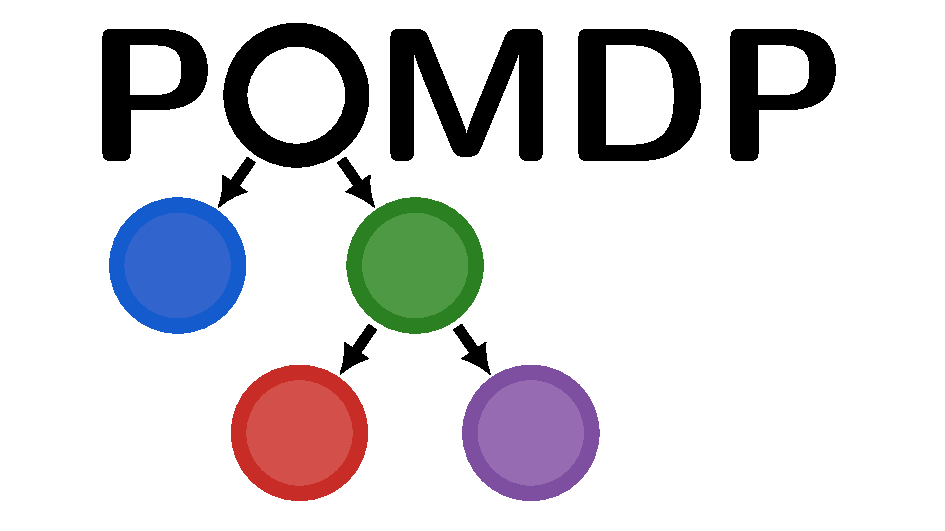
\includegraphics[height=3cm]{images/pomdps_logo.pdf}};
    % \node[xshift=-2cm, yshift=2cm] (img1) at (current page.south east) {\transduration<0-21>{0}\multiinclude[<+->][format=png, graphics={width=\textwidth}]{images/grid-world-animation/gridworld_value_iteration_γ}};
\end{tikzpicture}

\end{frame}

%-------------------------------------------------

\begin{frame}[fragile]{Example problems covered in this course}

Common problems in the literature are used as running examples.

% TODO: Photos.

{\footnotesize
\begin{itemize}
    \item \textbf{$^\text{(MDP)}$ Grid World}: Agent moving around a grid world, looking for rewards.
    \item \textbf{$^\text{(POMDP)}$ Crying Baby}: When to feed a baby, based on crying observations.
    \item \textbf{$^\text{(MDP)}$ 1D Random Walk}: Agent moves around the number line.
    \item \textbf{$^\text{(POMDP)}$ 2D Random Walk}: Estimating state of a moving agent based on observations.
    \item \textbf{$^\text{(MDP)}$ Mountain Car}: Reach a goal up a hill, starting in a valley.
    \item \textbf{$^\text{(MDP)}$ Swinging Pendulum}: Balance a swinging pendulum upright.
\end{itemize}
}

\begin{minipage}[b]{0.18\textwidth}
    \centering
    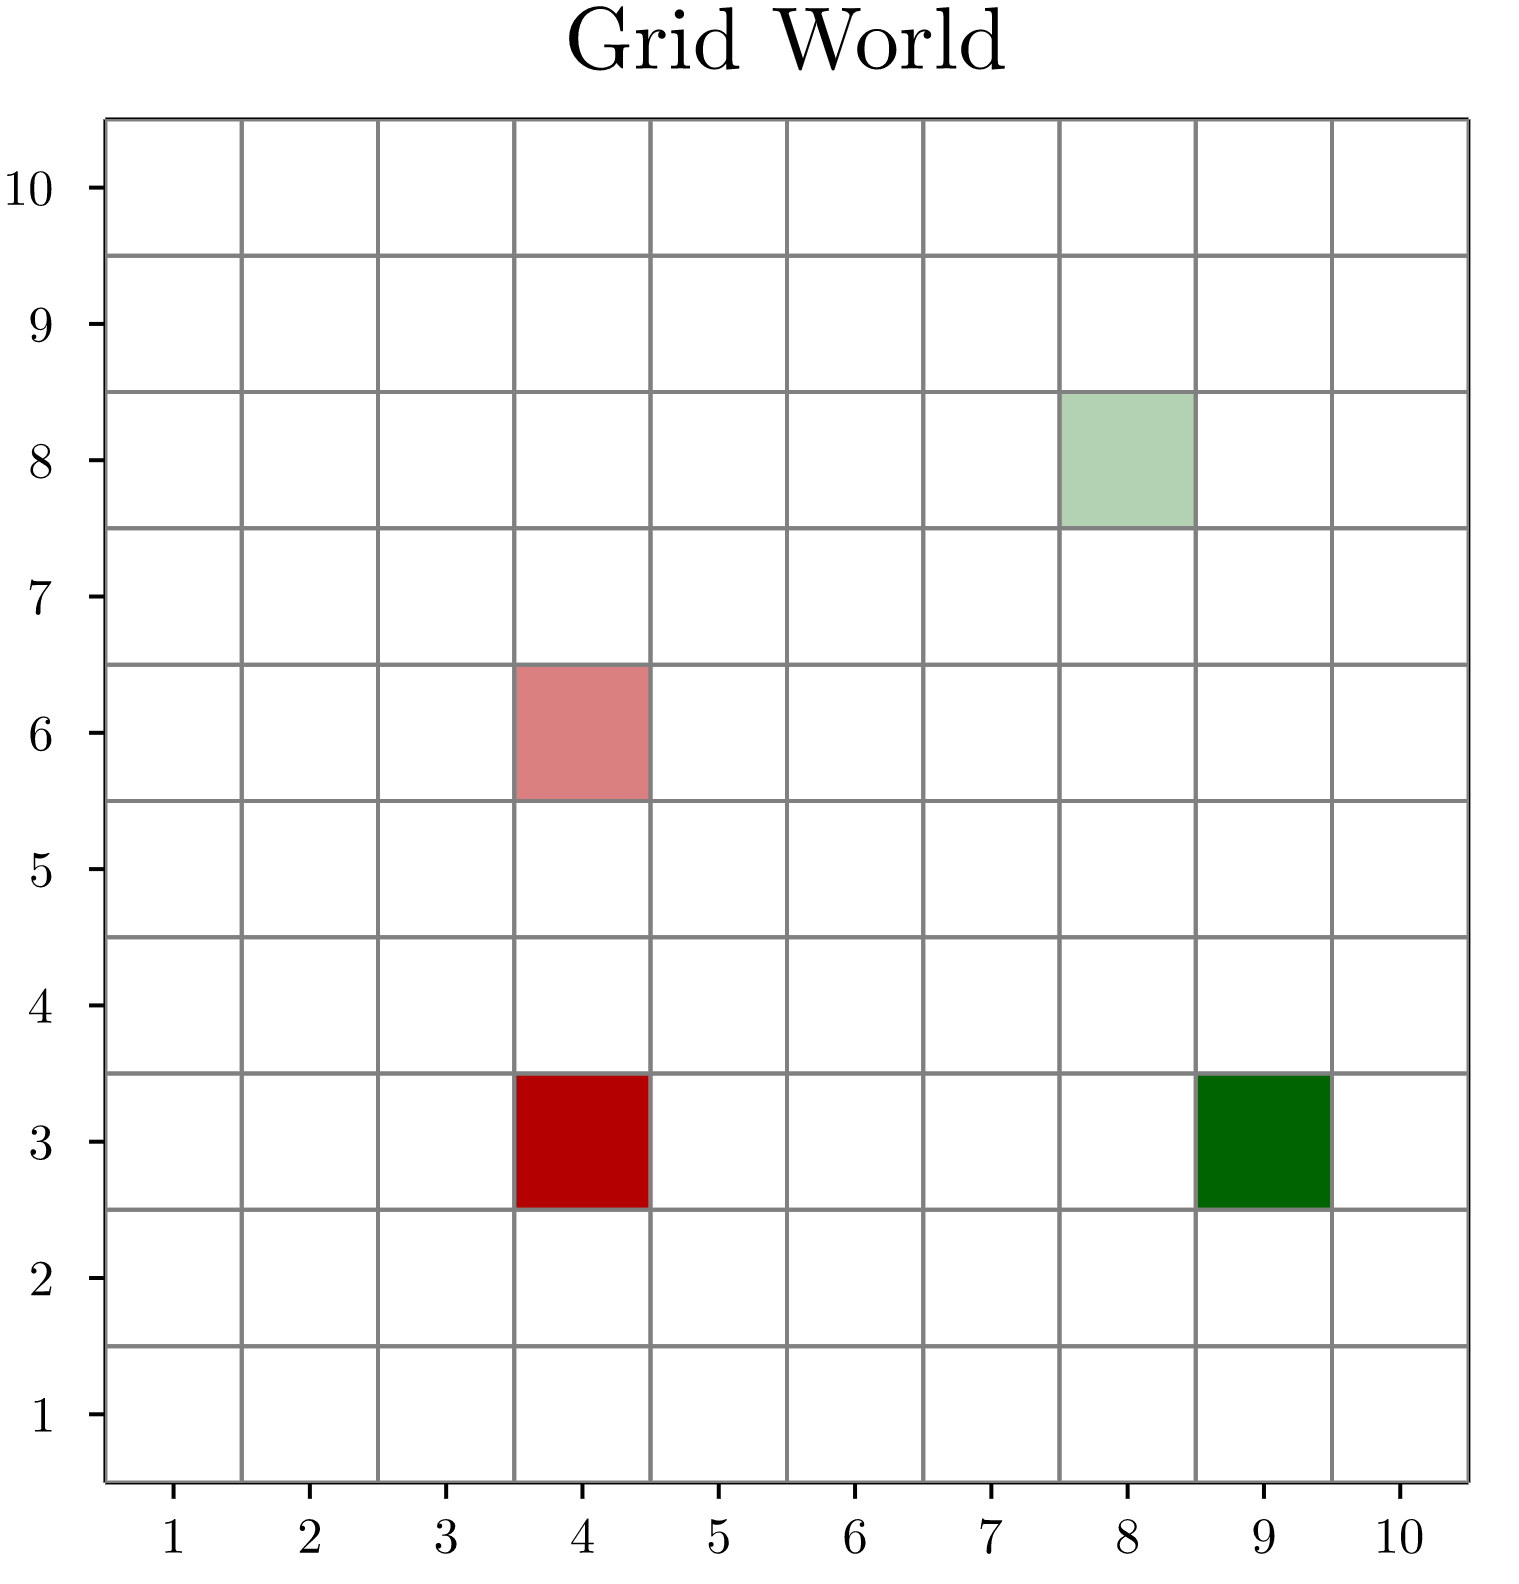
\includegraphics[align=c, width=0.8\textwidth]{images/grid-world.png}
\end{minipage}
\hfill
\begin{minipage}[b]{0.18\textwidth}
    \centering
    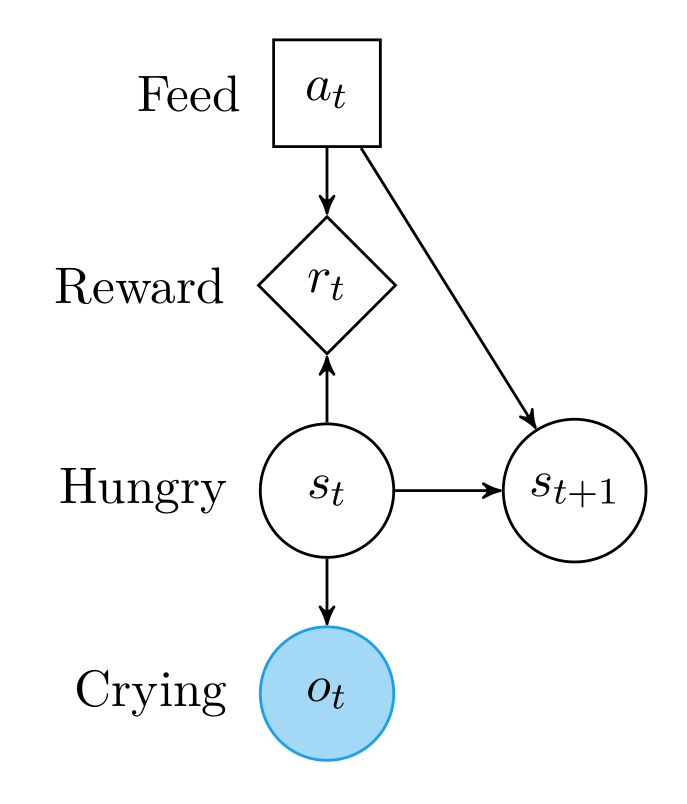
\includegraphics[align=c, width=0.9\textwidth]{images/crying-baby.png}
    % \resizebox{!}{0.3\textheight}{%
    % \begin{tikzpicture}
    %     \node[minimum size=1cm, draw=black, fill=white, circle] (s) {$s_t$};
    %     \node[minimum size=1cm, draw=black, fill=white, circle, right=0.8cm of s] (s2) {$s_{t+1}$};
    %     \node[minimum size=1cm, draw=pastelBlue, fill=pastelBlue!40, circle, below=0.5cm of s] (o) {$o_t$};
    %     \node[minimum size=1cm, draw=black, fill=white, diamond, above=0.5cm of s] (r) {$r_t$};
    %     \node[minimum size=0.8cm, draw=black, fill=white, rectangle, above=0.5cm of r] (a) {$a_t$};
    %     \node[left=0.1 of a, anchor=east] {Feed};
    %     \node[left=0.1 of r, anchor=east] {Reward};
    %     \node[left=0.1 of s, anchor=east] {Hungry};
    %     \node[left=0.1 of o, anchor=east] {Crying};
    %     \draw[->] (s) -- (o);
    %     \draw[->] (s) -- (s2);
    %     \draw[->] (s) -- (r);
    %     \draw[->] (a) -- (r);
    %     \draw[->] (a) -- (s2);
    % \end{tikzpicture}}
\end{minipage}
\hfill
\begin{minipage}[b]{0.18\textwidth}
    \centering
    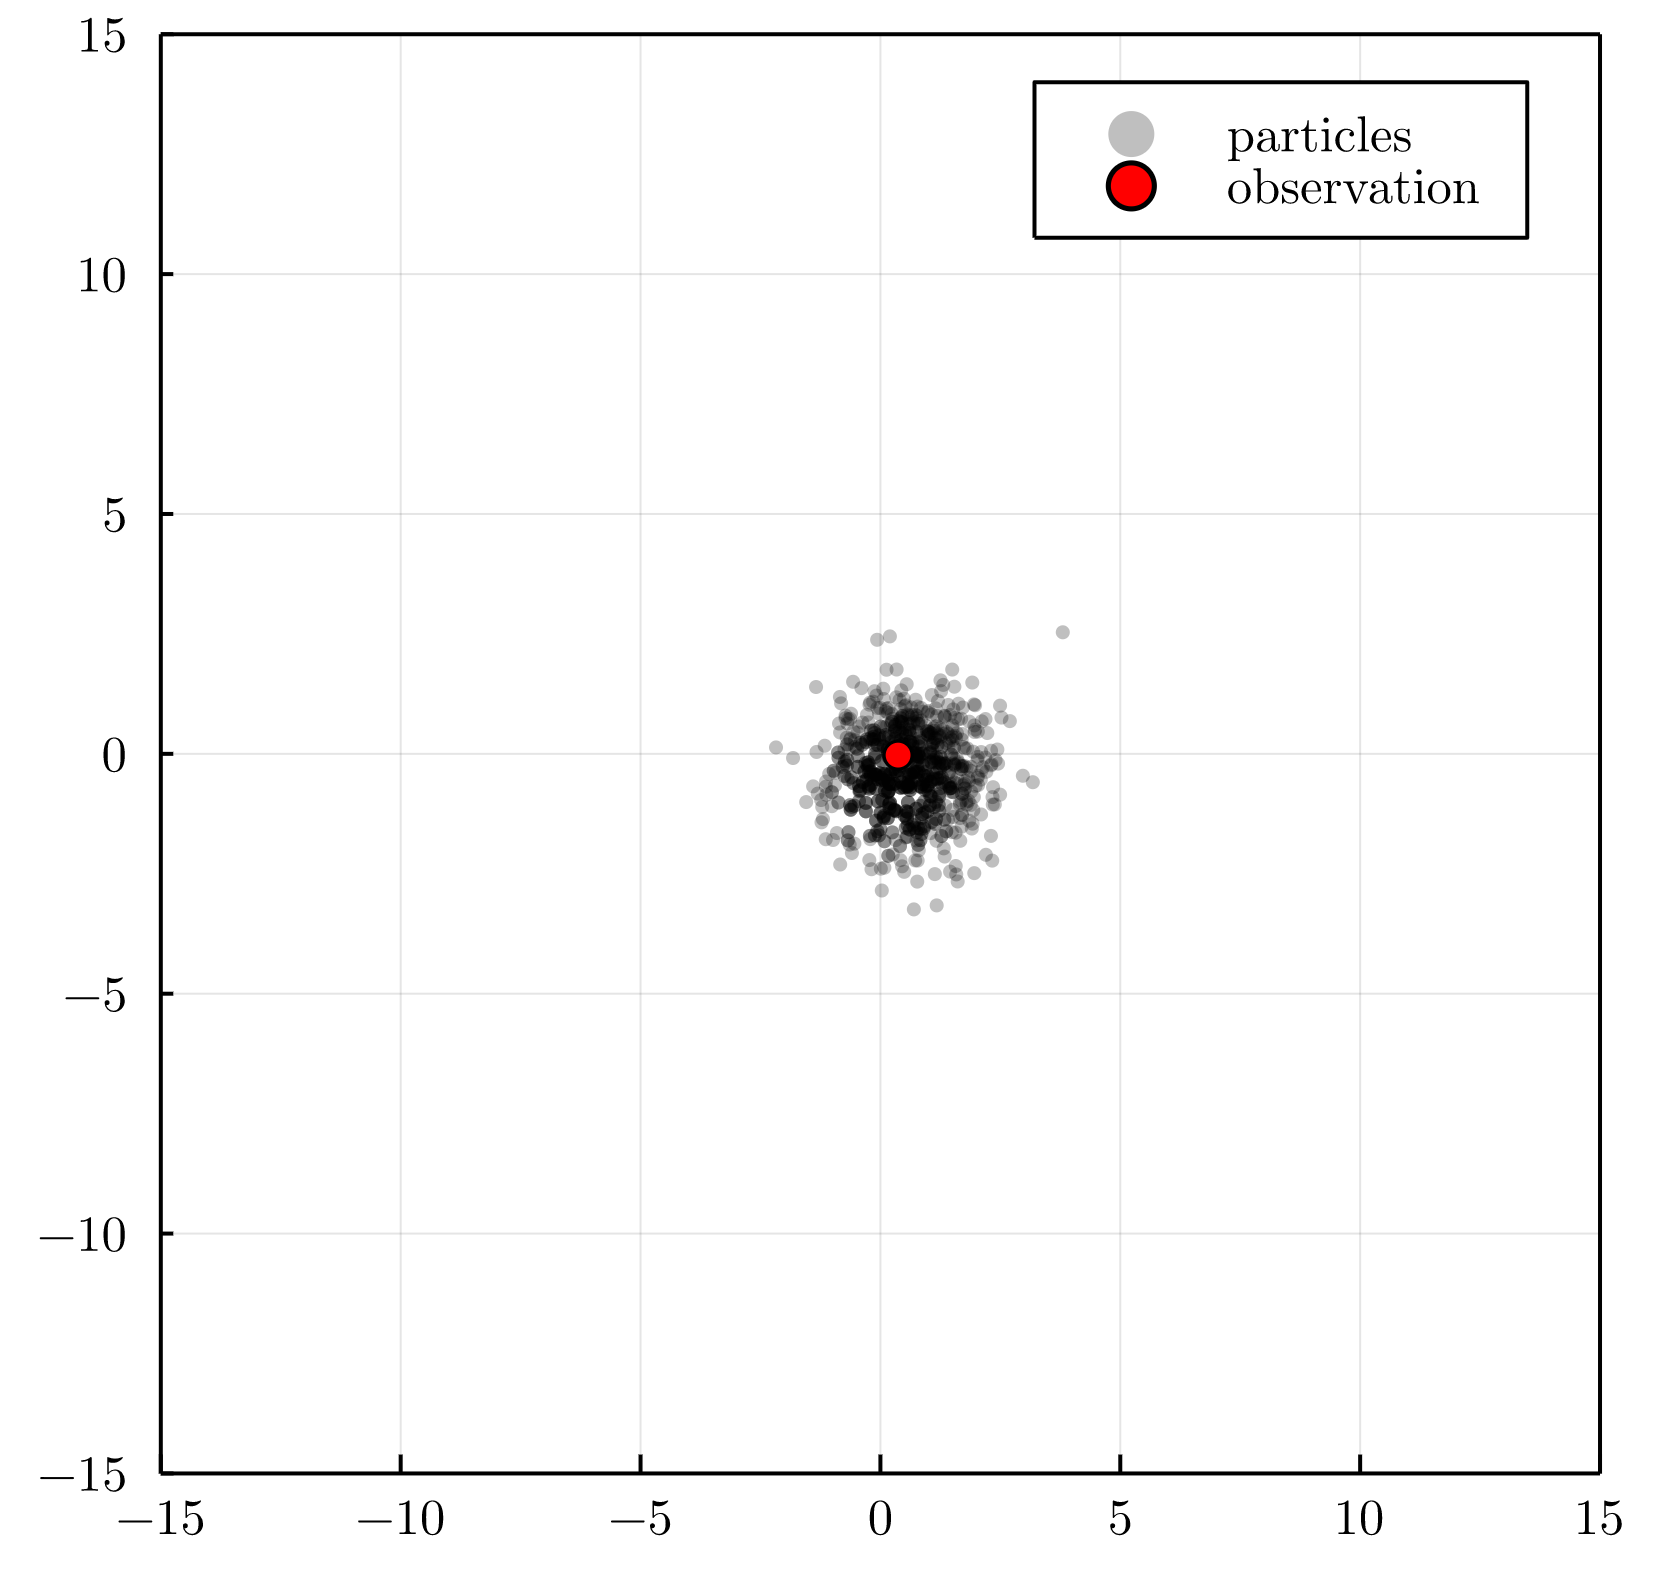
\includegraphics[align=c, width=1.0\textwidth]{images/particle-filter.png}
\end{minipage}
\hfill
\begin{minipage}[b]{0.18\textwidth}
    \centering
    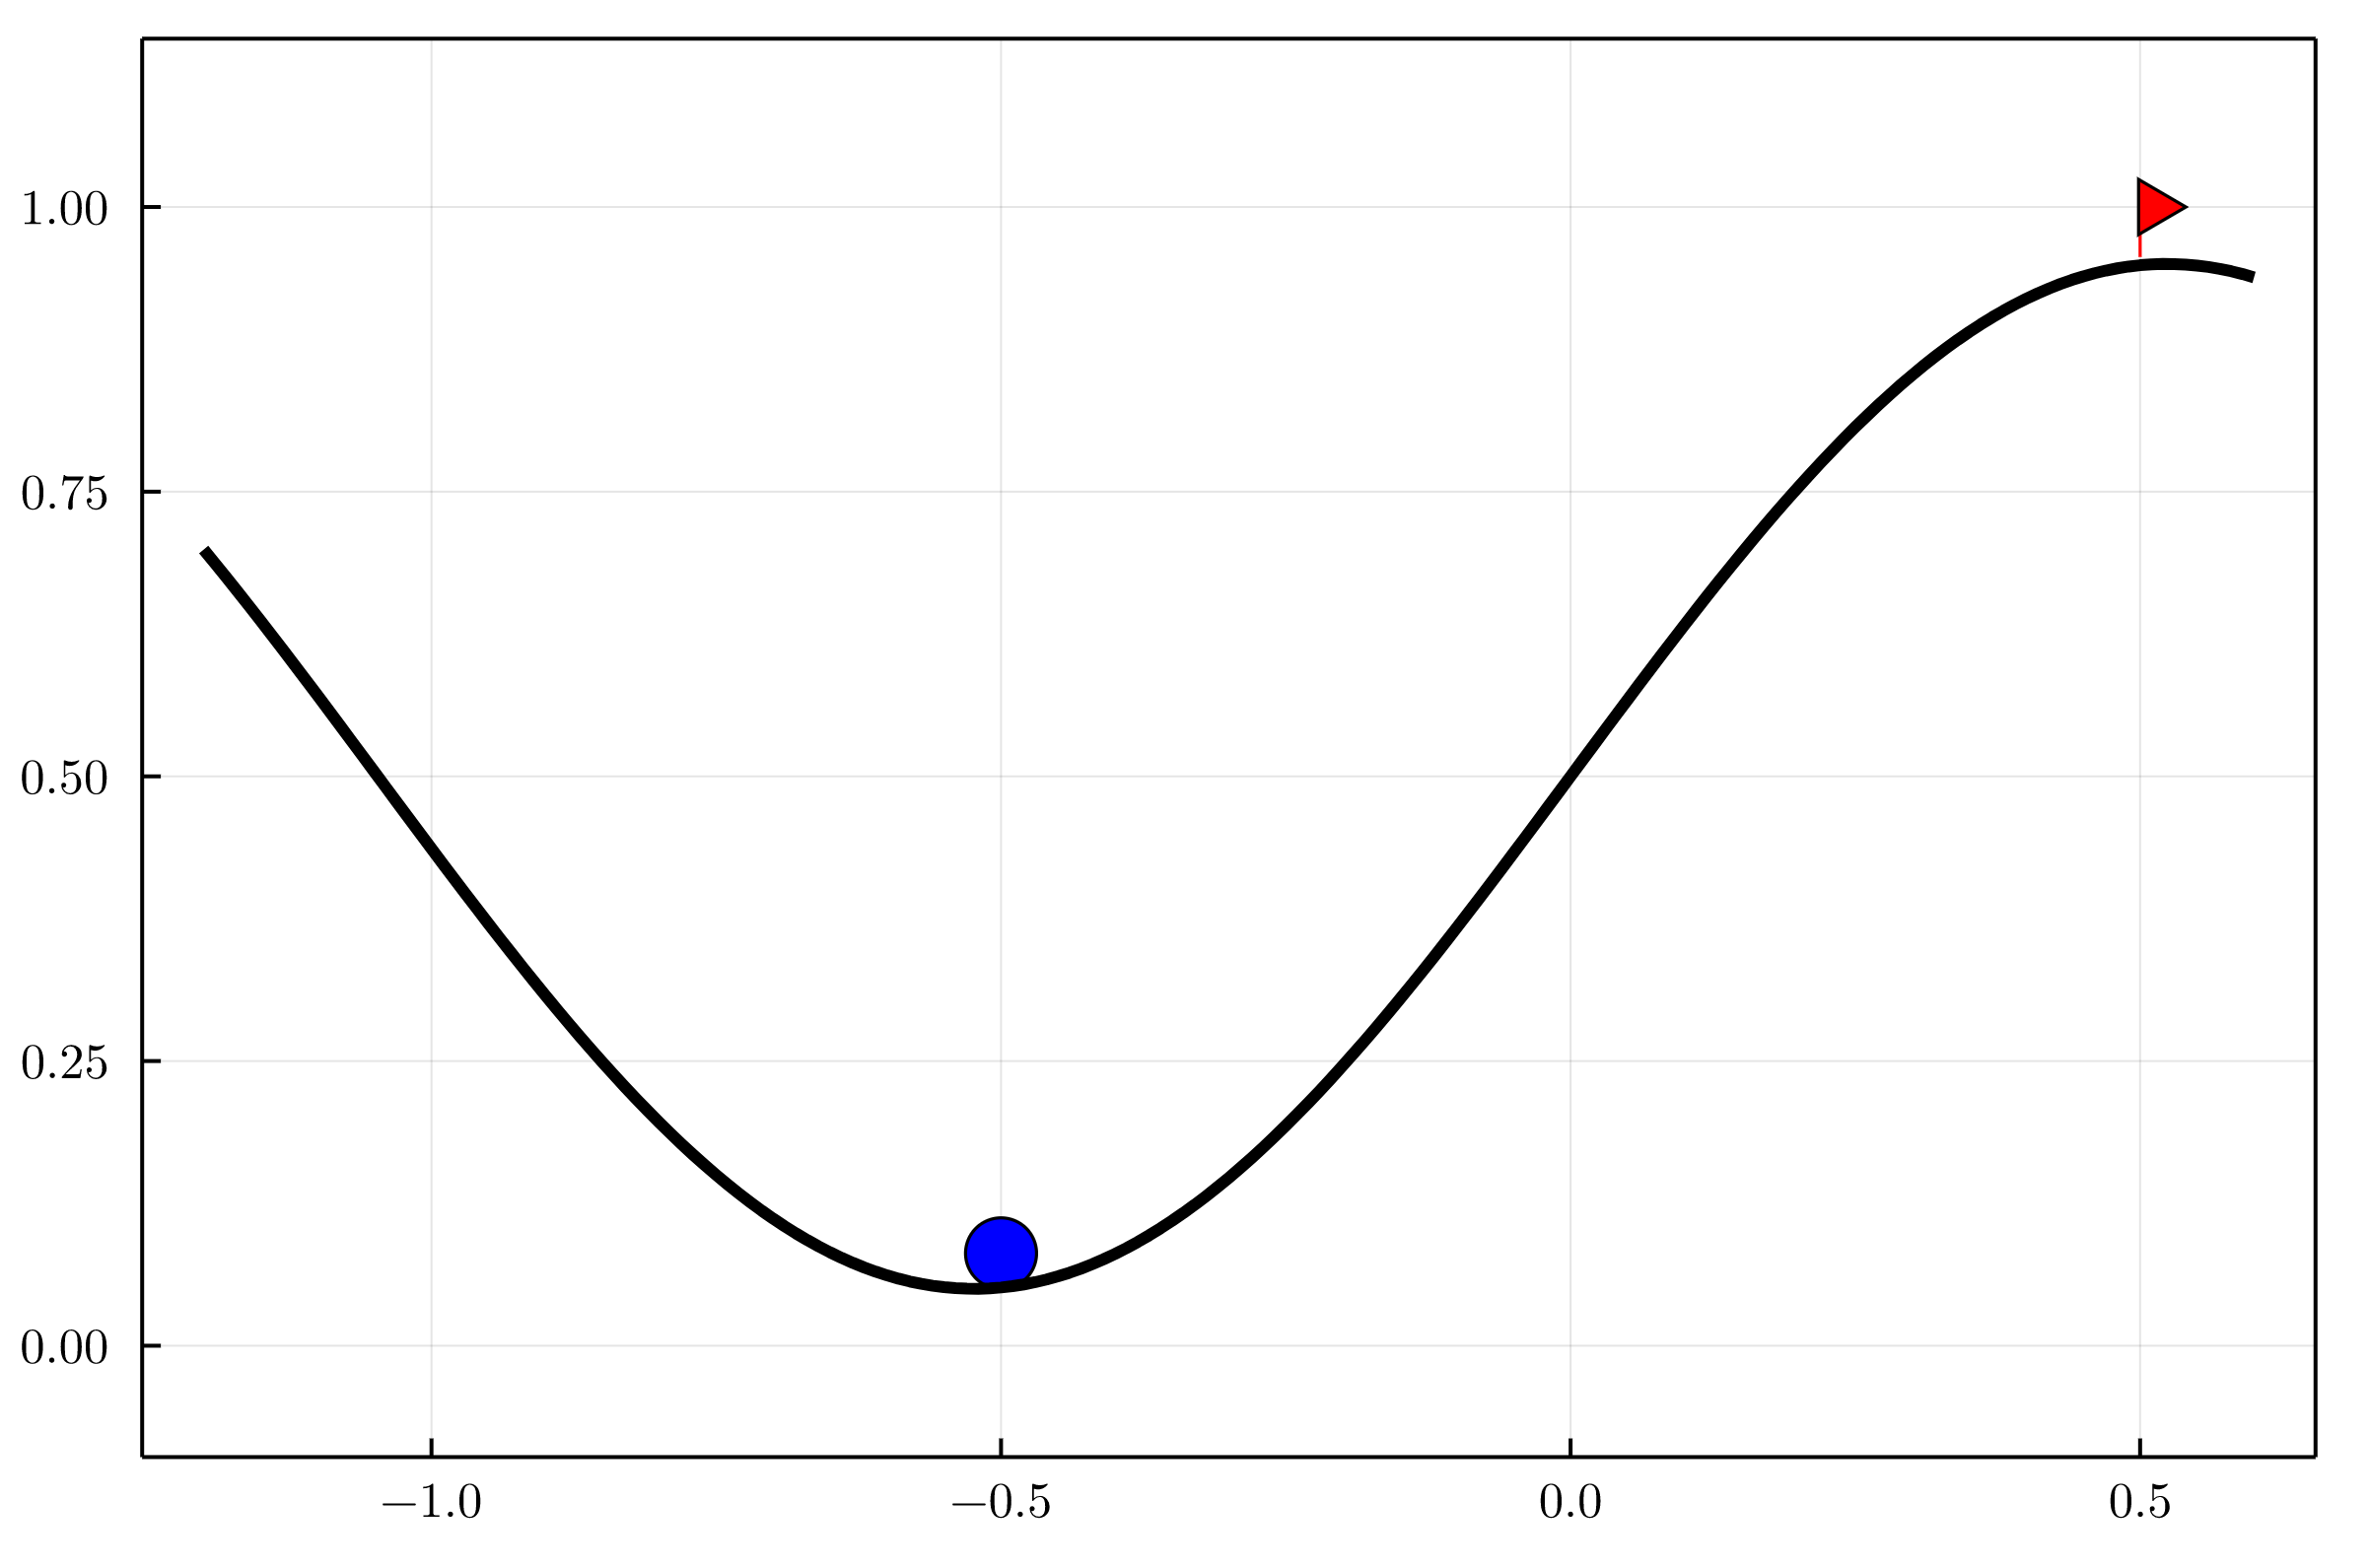
\includegraphics[align=c, width=1.0\textwidth]{images/mountain-car.png}
\end{minipage}
\hfill
\begin{minipage}[b]{0.18\textwidth}
    \centering
    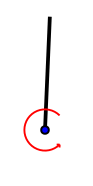
\includegraphics[align=c, width=0.5\textwidth]{images/pendulum.png}
\end{minipage}

\end{frame}

%-------------------------------------------------

\begin{frame}[fragile]{\texttt{POMDPs.jl} package ecosystem}

\begin{highlightblock}
The \texttt{POMDPs.jl} package itself contains the interface to define problem definitions.
\end{highlightblock}

\phantom{}

Other packages provide supporting tools that contain most of the functionality:\footnotemark[1]

\begin{columns}[T,onlytextwidth]
    \begin{column}{0.28\linewidth}
        {\tiny
        \begin{itemize}
            \item {\color{julia_blue}\href{https://github.com/JuliaPOMDP/QuickPOMDPs.jl}{\texttt{QuickPOMDPs.jl}}}
            \item {\color{julia_blue}\href{https://github.com/JuliaPOMDP/POMDPModelTools.jl}{\texttt{POMDPModelTools.jl}}}
            \item {\color{julia_blue}\href{https://github.com/JuliaPOMDP/POMDPPolicies.jl}{\texttt{POMDPPolicies.jl}}}
            \item {\color{julia_blue}\href{https://github.com/JuliaPOMDP/POMDPSimulators.jl}{\texttt{POMDPSimulators.jl}}}
            \item {\color{julia_blue}\href{https://github.com/JuliaPOMDP/POMDPModels.jl}{\texttt{POMDPModels.jl}}}
            \item {\color{julia_blue}\href{https://github.com/JuliaPOMDP/POMDPGallery.jl}{\texttt{POMDPGallery.jl}}}
            \item {\color{julia_green}\href{https://github.com/JuliaPOMDP/BeliefUpdaters.jl}{\texttt{BeliefUpdaters.jl}}}
            \item {\color{julia_green}\href{https://github.com/JuliaPOMDP/ParticleFilters.jl}{\texttt{ParticleFilters.jl}}}
            \item {\color{julia_green}\href{https://github.com/sisl/POMDPModelChecking.jl}{\texttt{POMDPModelChecking.jl}}}
            \item {\color{julia_green}\href{https://github.com/sisl/POMDPStressTesting.jl}{\texttt{POMDPStressTesting.jl}}}
        \end{itemize}
        }
    \end{column}
    \begin{column}{0.36\linewidth}
        {\tiny
        \begin{itemize}
            \item {\color{julia_red}\href{https://github.com/JuliaPOMDP/DiscreteValueIteration.jl}{\texttt{DiscreteValueIteration.jl}}}
            \item {\color{julia_red}\href{https://github.com/JuliaPOMDP/LocalApproximationValueIteration.jl}{\texttt{LocalApproximationValueIteration.jl}}}
            \item {\color{julia_red}\href{https://github.com/JuliaPOMDP/GlobalApproximationValueIteration.jl}{\texttt{GlobalApproximationValueIteration.jl}}}
            \item {\color{julia_red}\href{https://github.com/JuliaPOMDP/MCTS.jl}{\texttt{MCTS.jl}}}
            \item {\color{julia_red}\href{https://github.com/JuliaPOMDP/TabularTDLearning.jl}{\texttt{TabularTDLearning.jl}}}
            \item {\color{julia_red}\href{https://github.com/JuliaPOMDP/DeepQLearning.jl}{\texttt{DeepQLearning.jl}}}
            \item {\color{julia_red}\href{https://github.com/ancorso/Crux.jl}{\texttt{Crux.jl}}}
            \item {\color{julia_purple}\href{https://github.com/JuliaPOMDP/QMDP.jl}{\texttt{QMDP.jl}}}
            \item {\color{julia_purple}\href{https://github.com/JuliaPOMDP/FIB.jl}{\texttt{FIB.jl}}}
        \end{itemize}
        }
    \end{column}
    \begin{column}{0.32\linewidth}
        {\tiny
        \begin{itemize}
            \item {\color{julia_purple}\href{https://github.com/JuliaPOMDP/BeliefGridValueIteration.jl}{\texttt{BeliefGridValueIteration.jl}}}
            \item {\color{julia_purple}\href{https://github.com/JuliaPOMDP/SARSOP.jl}{\texttt{SARSOP.jl}}}
            \item {\color{julia_purple}\href{https://github.com/JuliaPOMDP/BasicPOMCP.jl}{\texttt{BasicPOMCP.jl}}}
            \item {\color{julia_purple}\href{https://github.com/JuliaPOMDP/ARDESPOT.jl}{\texttt{ARDESPOT.jl}}}
            \item {\color{julia_purple}\href{https://github.com/JuliaPOMDP/MCVI.jl}{\texttt{MCVI.jl}}}
            \item {\color{julia_purple}\href{https://github.com/JuliaPOMDP/POMDPSolve.jl}{\texttt{POMDPSolve.jl}}}
            \item {\color{julia_purple}\href{https://github.com/JuliaPOMDP/IncrementalPruning.jl}{\texttt{IncrementalPruning.jl}}}
            \item {\color{julia_purple}\href{https://github.com/JuliaPOMDP/POMCPOW.jl}{\texttt{POMCPOW.jl}}}
            \item {\color{julia_purple}\href{https://github.com/JuliaPOMDP/AEMS.jl}{\texttt{AEMS.jl}}}
            \item {\color{julia_purple}\href{https://github.com/JuliaPOMDP/PointBasedValueIteration.jl}{\texttt{PointBasedValueIteration.jl}}}
        \end{itemize}
        }
    \end{column}
\end{columns}

\footnotetext[1]{\textit{Key}: {\color{julia_blue}Tools}, {\color{julia_green}Extensions}, {\color{julia_red}MDP solvers}, {\color{julia_purple}POMDP solvers}.}

\end{frame}

%-------------------------------------------------

\begin{frame}[fragile]{Other resources}

There are many \textit{excellent} resources on MDPs/POMDPs and reinforcement learning:

{\scriptsize
\begin{itemize}
    \item \textbf{\textit{Algorithms for Decision Making}, Kochenderfer, Wheeler, \& Wray} ({\color{julia_blue}\url{https://algorithmsbook.com/}})
    \item \textbf{\textit{Reinforcement Learning: An Introduction}, Sutton \& Barto} ({\color{julia_blue}\url{http://incompleteideas.net/book/the-book.html}})
    \item \textbf{\textit{POMDPs.jl: A Framework for Sequential Decision Making under Uncertainty}, Egorov, Sunberg, et al., Journal of Machine Learning Research, 2017} ({\color{julia_blue}\url{https://www.jmlr.org/papers/volume18/16-300/16-300.pdf}})
    \item \textbf{Introduction to Reinforcement Learning with David Silver} ({\color{julia_blue}\url{https://deepmind.com/learning-resources/-introduction-reinforcement-learning-david-silver}})
\end{itemize}
}

\end{frame}

%-------------------------------------------------

\begin{frame}[fragile]{Observation space}


\begin{itemize}
    \item The agent receives an observation $o$, which belongs to some \textit{observation space} $\mathcal{O}$
    \item The probability of observing $o$ given action $a$ and next state $s^\prime$ is: $O(o \mid a, s^\prime)$
    \begin{itemize}
        \item If $\mathcal{O}$ is continuous, then $O(o \mid a, s^\prime)$ is a probability density
    \end{itemize}

\end{itemize}


\end{frame}



\begin{frame}[fragile]{Dynamic Decision Network for POMDPs}

\begin{figure}
    \centering
    \begin{tikzpicture}[x=1cm, y=1cm]
        \node[minimum size=1cm, draw=black, fill=white, circle] (s) {$s_t$};
        \node[minimum size=1cm, draw=black, fill=white, circle, right=1cm of s] (s2) {$s_{t+1}$};
        \node[minimum size=1cm, draw=pastelBlue, fill=pastelBlue!40, circle, below=0.5cm of s] (o) {$o_t$};
        \node[minimum size=1.3cm, draw=black, fill=white, diamond, above=0.5cm of s] (r) {$r_t$};
        \node[minimum size=1cm, draw=black, fill=white, rectangle, above=0.5cm of r] (a) {$a_t$};
        \node[minimum size=1cm, draw=black, fill=white, rectangle, left=1cm of a] (am1) {$a_{t-1}$};

        \node[minimum size=1.3cm, draw=lightgray, fill=white, diamond] (rm1) at (am1|-r) {\textcolor{lightgray}{$r_{t-1}$}};
        \node[minimum size=1cm,   draw=lightgray, fill=white, circle]  (sm1) at (am1|-s) {\textcolor{lightgray}{$s_{t-1}$}};
        \node[minimum size=1cm,   draw=lightgray, fill=white, circle]  (om1) at (am1|-o) {\textcolor{lightgray}{$o_{t-1}$}};

        \node[minimum size=1cm,   draw=lightgray, fill=white, rectangle] (ap1) at (s2|-a) {\textcolor{lightgray}{$a_{t+1}$}};
        \node[minimum size=1.3cm, draw=lightgray, fill=white, diamond]   (rp1) at (s2|-r) {\textcolor{lightgray}{$r_{t+1}$}};
        \node[minimum size=1cm,   draw=lightgray, fill=white, circle]    (op1) at (s2|-o) {\textcolor{lightgray}{$o_{t+1}$}};

        \draw[->] (s) -- (o);
        \draw[->] (s) -- (s2);
        \draw[->] (s) -- (r);
        \draw[->] (a) -- (r);
        \draw[->] (a) [out=0,in=135] to (s2);
        \draw[->] (am1) [out=0,in=135] to (o);
    \end{tikzpicture}
    \caption{
        \label{fig:su_beliefs_pomdp_trellis}
        A dynamic decision network for the POMDP problem formulation.
    }
\end{figure}

\end{frame}
\begin{frame}[fragile]{Dynamic Decision Network for POMDPs}

\begin{figure}
    \centering
    \begin{tikzpicture}[x=1cm, y=1cm]
        \node[minimum size=1cm, draw=black, fill=white, circle] (s) {$s_t$};
        \node[minimum size=1cm, draw=black, fill=white, circle, right=1cm of s] (s2) {$s_{t+1}$};
        \node[minimum size=1cm, draw=pastelBlue, fill=pastelBlue!40, circle, below=0.5cm of s] (o) {$o_t$};
        \node[minimum size=1.3cm, draw=black, fill=white, diamond, above=0.5cm of s] (r) {$r_t$};
        \node[minimum size=1cm, draw=black, fill=white, rectangle, above=0.5cm of r] (a) {$a_t$};
        \node[minimum size=1cm, draw=black, fill=white, rectangle, left=1cm of a] (am1) {$a_{t-1}$};

        \node[minimum size=1.3cm, draw=lightgray, fill=white, diamond] (rm1) at (am1|-r) {\textcolor{lightgray}{$r_{t-1}$}};
        \node[minimum size=1cm,   draw=lightgray, fill=white, circle]  (sm1) at (am1|-s) {\textcolor{lightgray}{$s_{t-1}$}};
        \node[minimum size=1cm,   draw=lightgray, fill=white, circle]  (om1) at (am1|-o) {\textcolor{lightgray}{$o_{t-1}$}};

        \node[minimum size=1cm,   draw=lightgray, fill=white, rectangle] (ap1) at (s2|-a) {\textcolor{lightgray}{$a_{t+1}$}};
        \node[minimum size=1.3cm, draw=lightgray, fill=white, diamond]   (rp1) at (s2|-r) {\textcolor{lightgray}{$r_{t+1}$}};
        \node[minimum size=1cm,   draw=lightgray, fill=white, circle]    (op1) at (s2|-o) {\textcolor{lightgray}{$o_{t+1}$}};

        \draw[->] (s) -- (o);
        \draw[->] (s) -- (s2);
        \draw[->] (s) -- (r);
        \draw[->] (a) -- (r);
        \draw[->] (a) [out=0,in=135] to (s2);
        \draw[->] (am1) [out=0,in=135] to (o);
    \end{tikzpicture}
    \caption{
        \label{fig:su_beliefs_pomdp_trellis}
        A dynamic decision network for the POMDP problem formulation.
    }
\end{figure}

\end{frame}

\begin{frame}[fragile]{Belief Representation}

Beliefs can be represented in different ways:
\begin{itemize}
    \item \textbf{Parametric}: The belief distribution is represented by a set of parameters for a fixed distribution family
    \begin{itemize}
        \item E.g., Categorical distribution\footnote{A probability mass is assigned to each discrete category.} or multivariate normal (Gaussian) distribution
    \end{itemize}
    \item \textbf{Non-parametric}: The belief distribution is represented by particles (or points sampled from the state space)
\end{itemize}

\vspace{5mm}
Depending on the representation, different algorithms can be used to update beliefs.


\end{frame}

\begin{frame}{Algorithms for Updating Beliefs}

Various algorithms can update the current belief:
\begin{itemize}
    \item If the state space is \textit{discrete} (or certain linear Gaussian assumptions are met), then we can perform \textit{exact belief updates}:\footnote{Meaning we arrive at an analytical solution without approximations.}
    \begin{itemize}
        \item Recursive Bayesian estimation (i.e. discrete state filter)
        \item Kalman filter
    \end{itemize}
    \item Otherwise, we can use approximations based on linearization or sampling:
    \begin{itemize}
        \item Extended Kalman filter
        \item Unscented Kalman filter
        \item Particle filter
        \item Particle filter with rejection
        \item Injection particle filter
        \item Adaptive injection particle filter
    \end{itemize}
\end{itemize}

\end{frame}
\begin{frame}[fragile]{Belief Initialization}

Before any actions or observations, we start with an initial belief distribution
\begin{itemize}
    \item We can encode prior knowledge in the initial distribution
    \item Generally want to use diffuse (i.e. spread out) initial distributions to avoid over confidence in the absence of information
    \begin{itemize}
        \item In non-parametric representations, a diffuse initial prior may cause difficulties
        \item Thus, we may wait until an informative observation is make to initialize beliefs
    \end{itemize}
\end{itemize}


\end{frame}




\begin{frame}[fragile]{Example: Landmark Belief Initialization}

\begin{figure}
    \caption{Localization of an autonomous car using a landmark (Example 19.1).}
    \begin{center}
        \begin{jlcode}
            p = let
                Random.seed!(0)

                tikz_string = ""
                tikz_string *= "\\coordinate (ego) at (1,-0.3);\n"
                tikz_string *= "\\draw [rounded corners=1] (\$(ego) - (0.5,0.25)\$) rectangle ++(1,0.5);\n"
                tikz_string *= "\\coordinate (sensor) at (\$(ego) + (0.25,0)\$);\n"
                tikz_string *= "\\def\\ang{12}\n"
                tikz_string *= "\\def\\r{5}\n"
                tikz_string *= "\\coordinate (landmark) at (\$(sensor) + (\\ang:\\r)\$);\n"
                tikz_string *= "\\draw (landmark) circle (0.5);\n"
                tikz_string *= "\\node[anchor=south, font=\\footnotesize] at (\$(landmark) + (0,0.5)\$) {landmark};\n"
                tikz_string *= "\\draw[thick, pastelBlue] (sensor) -- (landmark);\n"
                tikz_string *= "\\fill[pastelBlue] (landmark) circle (0.1);\n\n"

                tikz_string *= "\\node[anchor=south, font=\\tiny] at (\$(sensor)!0.5!(landmark)\$) {\$r\$};"
                tikz_string *= "\\def\\rarc{3}"
                tikz_string *= "\\draw[-{stealth[length=1mm,width=0.5mm]}] (\$(sensor) + (0:\\rarc)\$) arc (0:\\ang:\\rarc);"
                tikz_string *= "\\node[anchor=west, font=\\tiny] at (\$(sensor) + (\\ang/2:\\rarc)\$) {\$\\theta\$};"

                r = 5
                θ = deg2rad(12)
                νr = 0.5
                νθ = 0.1
                Gr = Normal(r, νr)
                Gθ = Normal(θ, νθ)
                Uϕ = Uniform(0.0, 2π)

                landmark_x = 0.5 + r*cos(θ)
                landmark_y = -0.55 + r*sin(θ)

                for i in 1:100
                    r_hat = rand(Gr)
                    θ_hat = rand(Gθ)
                    ϕ_hat = rand(Uϕ)
                    car_x = landmark_x - r_hat * cos(θ_hat)
                    car_y = landmark_y - r_hat * sin(θ_hat)

                    tikz_string *= "\\draw [opacity=0.2, rotate around={$(rad2deg(ϕ_hat)):(landmark)}, rounded corners=1] ($(car_x),$(car_y)) rectangle ++(1,0.5);\n"
                end

                TikzPicture(tikz_string, preamble="", options="x=0.4cm, y=0.4cm")
            end
            plot(p)
        \end{jlcode}
        \plot{fig/sample_from_induced_landmark_obs}
    \end{center}
\end{figure}

{\small Making a range $r$ and bearing $\theta$ observation, we initialize our belief around the landmark.}

\end{frame}
\begin{frame}[fragile]{Belief Inference}

\begin{itemize}
    \item To infer the unknown belief distribution, we use \textit{recursive Bayesian estimation}
    \begin{itemize}
        \item Updates belief estimate recursively over time
        \item Markov assumption: Only requires the current state, action, and observation
    \end{itemize}
    \item Let $b(s)$ represent the probability\footnote{or probability density for continuous state spaces} assigned to state $s$
    \begin{itemize}
        \item A particular belief $b$ belongs to a \textit{belief space} $\mathcal{B}$ (which contains all possible beliefs)
    \end{itemize}
    \item For finite state and observation spaces, we can use a \textit{discrete state filter} to perform exact inference
\end{itemize}


\end{frame}
\begin{frame}[fragile]{Belief Vector}

\begin{itemize}
    \item In the finite state case, we can represent beliefs using a categorical distribution\footnote{A probability mass is assigned to each discrete state.}
    \begin{itemize}
        \item Represented as a \textit{belief vector} $\vec{b}$ of length $\card{\mathcal{S}}$, therefore $\mathcal{B} \subset \R^{\card{\mathcal{S}}}$
        \item Sometimes $\mathcal{B}$ is referred to as a \textit{probability simplex} or \textit{belief simplex}\footnote{Simplex being the generalization of a triangle to arbitrary dimensions.}
    \end{itemize}
\end{itemize}

% \vspace{5mm}

\begin{itemize}
    \item The belief vector $\vec{b}$ must be strictly non-negative and sum to one:
    \begin{equation*}
        b(s) \ge 0 \text{ for all } s \in \mathcal{S} \qquad \sum_s b(s) = 1
    \end{equation*}
    \item In vector notation:
    \begin{equation*}
        \vec{b} \ge \vec{0} \qquad \vec{1}^\top \vec{b} = 1
    \end{equation*}
    \item In Julia syntax:
\begin{center}
\jlv{all(𝐛 .≥ 0) && sum(𝐛) ≈ 1}
\end{center}
\end{itemize}

\end{frame}
\begin{frame}[fragile]{Discrete State Filter: Updating Beliefs}

% \begin{definitionblock}{Filter}
% A process that remove noise from data.\footnote{Often used in signal processing, effectively ``filtering'' out the noise.}
% \end{definitionblock}
A \textit{filter} is a process that remove noise from data.\footnote{Often used in signal processing, effectively ``filtering'' out the noise.}

\vspace{5mm}

Due to the independece assumptions, if an agent with belief $b$ takes an action $a$ and receives an observation $o$, then the new belief $b^\prime$ becomes:\footnote{For finite/discrete state and observation spaces.}
\begin{align*}
    b^\prime(s^\prime) &= P(s^\prime \mid b, a, o)\\
                       &\propto P(o \mid b, a, s^\prime) P(s^\prime \mid b, a) \tag{Bayes' rule}\\
                       &\propto O(o \mid a, s^\prime) P(s^\prime \mid b, a)\tag{observation definition}\\
                       &\propto O(o \mid a, s^\prime) \sum_s P(s^\prime \mid b, a, s) P(s \mid b, a) \tag{law of total probability}\\
                       &\propto O(o \mid a, s^\prime)\sum_s T(s^\prime \mid s, a)b(s) \tag{state transition model}
\end{align*}


\end{frame}
\begin{frame}[fragile]{Updating Beliefs: Derivation Explained}

\begin{align*}
    b^\prime(s^\prime) &= P(s^\prime \mid b, a, o) \tag{probability of being in state $s^\prime$}\\
                       &\propto P(o \mid b, a, s^\prime) P(s^\prime \mid b, a) \tag{Bayes' rule, dropping normalization}\\
                       &\propto O(o \mid a, s^\prime) P(s^\prime \mid b, a)\tag{observation model def., $o$ independent of $b$}\\
                       &\propto O(o \mid a, s^\prime) \sum_s P(s^\prime \mid b, a, s) P(s \mid b, a) \tag{law of total probability}\\
                       &\propto O(o \mid a, s^\prime)\sum_s T(s^\prime \mid s, a)b(s) \tag{state transition model, belief def.}
\end{align*}

\hrule

\vspace{5mm}

\begin{equation*}
    \textbf{Exact belief updating:}\footnote{Then normalize so beliefs sum to one.}\quad b^\prime(s^\prime) \propto O(o \mid a, s^\prime)\sum_s T(s^\prime \mid s, a)b(s)
\end{equation*}


\end{frame}
\begin{frame}[fragile]{Example: Crying Baby Problem}

\begin{columns}[T,onlytextwidth]
    \begin{column}{0.55\columnwidth}
        \begin{figure}
            \centering
            \begin{tikzpicture}
                \node[minimum size=1cm, draw=black, fill=white, circle] (s) {$s_t$};
                \node[minimum size=1cm, draw=black, fill=white, circle, right=0.8cm of s] (s2) {$s_{t+1}$};
                \node[minimum size=1cm, draw=pastelBlue, fill=pastelBlue!40, circle, below=0.5cm of s] (o) {$o_t$};
                \node[minimum size=1cm, draw=black, fill=white, diamond, above=0.5cm of s] (r) {$r_t$};
                \node[minimum size=0.8cm, draw=black, fill=white, rectangle, above=0.5cm of r] (a) {$a_t$};
                \node[left=0.1 of a, anchor=east] {Feed};
                \node[left=0.1 of r, anchor=east] {Reward};
                \node[left=0.1 of s, anchor=east] {Hungry};
                \node[left=0.1 of o, anchor=east] {Crying};
                \draw[->] (s) -- (o);
                \draw[->] (s) -- (s2);
                \draw[->] (s) -- (r);
                \draw[->] (a) -- (r);
                \draw[->] (a) -- (s2);
            \end{tikzpicture}
            \caption{
                \label{fig:crying_baby_pomdp}
                The crying baby POMDP.
            }
        \end{figure}
    \end{column}
    \begin{column}{0.45\columnwidth}
        \begin{itemize}
            \item A simple POMDP with 2 states, 3 actions, and 2 observations:
            \begin{align*}
                \mathcal{S} &= \{\text{hungry},\, \text{sated}\}\\
                \mathcal{A} &= \{\text{feed},\, \text{sing},\, \text{ignore}\}\\
                \mathcal{O} &= \{\text{crying},\, \text{quiet}\}
            \end{align*}
            \item See Pluto notebook:
            \begin{itemize}
                \item \href{http://htmlpreview.github.io/?https://raw.githubusercontent.com/mossr/StateEstimation.jl/master/html/crying_baby_problem.html}{\color{cardinal}crying\_baby\_problem.html}
            \end{itemize}
        \end{itemize}
    \end{column}
\end{columns}

\end{frame}
\begin{frame}[fragile]{Kalman Filter}

% \begin{definitionblock}{Filter}
% A process that remove noise from data.\footnote{Often used in signal processing, effectively ``filtering'' out the noise.}
% \end{definitionblock}
To update beliefs with \textit{continuous} state spaces, we integrate instead of sum:
\begin{gather*}
    b^\prime(s^\prime) \propto O(o \mid a, s^\prime)\int T(s^\prime \mid s, a)b(s)\;ds    
\end{gather*}

A \textit{Kalman filter} assumes that $T$ and $O$ are linear-Gaussian and $b$ is Gaussian:
\begin{align*}
    T(\mathbf{s}^\prime \mid \mathbf s, \mathbf a) &= \mathcal{N}(\mathbf{s}^\prime \mid \mathbf{T}_s \mathbf{s} + \mathbf{T}_a \mathbf{a},\, \mat{\Sigma}_s)\\
    O(\mathbf o \mid \mathbf{s}^\prime) &= \mathcal{N}(\mathbf o \mid \mathbf{O}_s \mathbf{s}^\prime,\, \mat{\Sigma}_o)\\
    b(\mathbf{s}) &= \mathcal{N}(\mathbf{s} \mid \vec{\mu}_b,\, \mat{\Sigma}_b)
\end{align*}

% \vspace{5mm}

See Pluto notebook: \href{http://htmlpreview.github.io/?https://raw.githubusercontent.com/mossr/StateEstimation.jl/master/html/kalman_filter.html}{\color{cardinal}StateEstimation.jl/kalman\_filter.html}

\end{frame}
% \include{slides/aa228/extended-kalman-filter}
% \include{slides/aa228/unscented-kalman-filter}
\begin{frame}[fragile]{Particle Filter}

% \begin{definitionblock}{Filter}
% A process that remove noise from data.\footnote{Often used in signal processing, effectively ``filtering'' out the noise.}
% \end{definitionblock}

\begin{itemize}
    \item \textit{Particle filters} represent the belief state as a collection of states.
    \item Each state in the approximated belief is called a \textit{particle}.
    \item Useful in problems with large discrete states spaces or continuous problems not well approximated by linear-Gaussian dynamics.
\end{itemize}

\begin{algorithm}[H]
    \caption{Particle filter algorithm.}
    \label{alg:particle_filter}
    \begin{algorithmic}
    \Function{ParticleFilter$(\mathbf{b}, T, O, a, o)$}{}
    \State $\mathbf{s}^\prime \sim T(\mathbf{b}, a)$ \algorithmiccomment{next states}
    \State $\mathbf{w} \leftarrow O(o \mid \mathbf{s}^\prime, a)$ \algorithmiccomment{weights}
    \State $\text{particles} \sim \operatorname{SetCategorical}\left(\mathbf{s}^\prime, \frac{\mathbf{w}}{\sum_i w_i}\right)$ \algorithmiccomment{sample with normalized weights}
    \State \Return $\text{particles}$
    \EndFunction
    \end{algorithmic}
\end{algorithm}

See Pluto notebook: \href{http://htmlpreview.github.io/?https://raw.githubusercontent.com/mossr/StateEstimation.jl/master/html/particle_filter.html}{\color{cardinal}StateEstimation.jl/particle\_filter.html}

\end{frame}
\begin{frame}[fragile]{Particle Filter Variants}

\textbf{Particle filter with rejection}:
\begin{itemize}
    \item Used in problems with discrete observations.
    \item Any sampled observation that does not equal the true observation is rejected.
    \item Problem of \textit{particle deprivation}: lack of particles near the true state.\footnote{Due to low particle coverage given the stochastic nature of resampling.}
\end{itemize}

\vspace{5mm}
\textbf{Injection particle filter}:
\begin{itemize}
    \item Inject random particles to protect against particle deprivation.
\end{itemize}

\vspace{5mm}
\textbf{Adaptive injection particle filter}:
\begin{itemize}
    \item Inject particles adaptively based on a ratio of two exponentially moving averages of the mean particle weights (using \textit{fast} and \textit{slow} moving averages).
\end{itemize}

\vspace{2mm}
See Pluto notebook: \href{http://htmlpreview.github.io/?https://raw.githubusercontent.com/mossr/StateEstimation.jl/master/html/particle_filter.html}{\color{cardinal}StateEstimation.jl/particle\_filter.html}

\end{frame}
% \include{slides/aa228/belief-summary}

% Chapter 20: Exact Belief State Planning
\section{Exact Belief State Planning}
\begin{frame}[fragile]{Introduction: Planning}

\begin{itemize}
    \item The objective in a POMDP is to maximize accumulated reward while interacting with the environment.
    \item Several methods can compute an optimal policy which maps \textit{beliefs} to \textit{actions}:
    \begin{itemize}
         \item One approach converts the POMDP into an MDP and applies dynamic programming.\footnote{Introducing an algorithm that is analogous to MDP value iteration.}
         \item Another approach represents policies as conditional plans or piecewise linear value functions over the belief space.
     \end{itemize} 
\end{itemize}

\end{frame}
% \include{slides/aa228/belief-state-mdp}
% \include{slides/aa228/conditional-plans}
% \include{slides/aa228/alpha-vectors}
% \include{slides/aa228/pomdp-value-iteration}
% \include{slides/aa228/linear-policies}
% \include{slides/aa228/planning-summary}




\begin{frame}{References}
    \renewcommand*{\bibfont}{\scriptsize}
    \printbibliography
\end{frame}

\end{document}